\documentclass[oneside]{book}
\usepackage[total={18cm, 21cm}, top=2cm, left=2cm]{geometry}
\parindent = 0mm % sin sangría
\usepackage{latexsym, amsmath, amssymb, amsfonts}
\usepackage[utf8]{inputenc}
\usepackage{graphicx}
\usepackage[spanish]{babel}
\usepackage{float}
\usepackage{longtable, multirow, booktabs}
\usepackage{caption}
\usepackage{makecell}
\usepackage{hyperref}
\begin{document}
\chapter{Using MQTT Over WebSockets with Mosquitto}
\url{http://www.steves-internet-guide.com/mqtt-websockets/}
\section{What is websockets and How it Works ?}
WebSocket is a computer communications protocol, providing full-duplex communication channels over a single TCP/IP connection.
\\\\
It is closely associated with http and it uses http for the initial connection establishment.
\\\\
The client and server connect using http and then negotiate a connection upgrade to websockets, the connection then switches from http to websockets.
\\\\
The client and server can now exchange full duplex binary data over the connection.

\section{Why Use MQTT over Websockets?}
MQTT over Websockets allows you to receive MQTT data directly into a web browser.
\\\\
This is important as the web browser may become the DE-facto interface for displaying MQTT data.
\\\\
MQTT websocket support for web browsers is provided by the JavaScript client.

\section{MQTT Over Websockets vs MQTT.}
In the case of MQTT over Websockets the websockets connection forms an outer pipe for the MQTT protocol.
\\\\
The  MQTT broker places the MQTT packet into a websockets packet, and sends it to the client.
\\\\
The client unpacks the MQTT packet from the websockets packet and then processes it as a normal MQTT packet.

\begin{figure}[H]
\centering
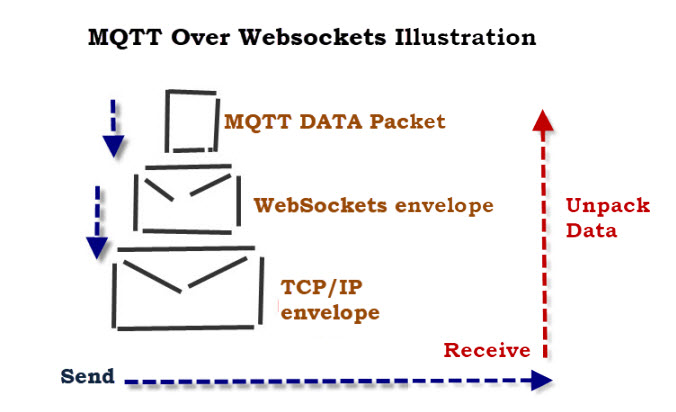
\includegraphics[scale=1]{images/mqtt_websocket.jpg}
\end{figure}
With MQTT the MQTT Packet is placed directly into the TCP/IP Packet.

\section{Websockets and Mosquitto}
The default Mosquitto install packages for Windows and Linux both support WebSockets.
\\\\
Very early versions 1.4.x needed to be compiled with websocket support. This is no longer necessary.	

\subsection{Websockets on Windows}
Since mosquitto 1.5.1 websockets support has been enabled on the windows binary files.
\\\\
However when you start mosquitto it appears to be listening on the websocket port but doesn’t allow connections.

\subsection{Configuring Websockets On Your Own Mosquitto Broker}
MQTT over Websockets usually uses port 9001 but it isn’t fixed.
\\\\
You need to make change to the mosquitto.conf file, by adding the following:
\begin{figure}[H]
\centering
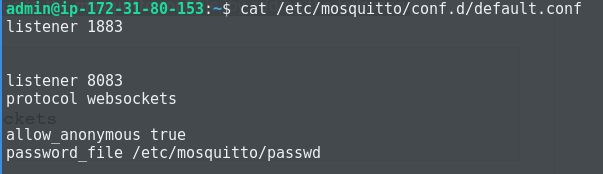
\includegraphics[scale=1]{images/mosquitto_setup.jpg}
\caption{Configuración Mosquitto}
\end{figure}

This creates an extra listener using websockets and port 8083.

\chapter{How to enable Mosquitto MQTT over WebSocket on Windows}
\url{https://iot4beginners.com/how-to-enable-mosquitto-mqtt-over-websocket-on-windows/}


WebSocket is one of the communication protocols which provides full duplex communication over a single TCP/IP connection. It uses HTTP as a initial connection establishment. The WebSocket enables the communication from the web browser (client) to the server, in which you can send some data or a real-time data to the client from the server or even bidirectional. At first, the client and the server interacts with HTTP, then the connection upgrades to the WebSocket, providing full duplex communication unlike HTTP. 
\\\\
HTTP Protocol always use long polling, but Websockets overcomes this problem. Because, the HTTP protocol always sends the data on request/response, and the WebSockets allows the server to send the data to the web browser or the client, even without any request from the browser. So, 2-way client server communication is possible with WebSockets.
\\\\
In this tutorial, we will learn how to enable MQTT over WebSocket on your windows machine. I have used Mosquitto Broker in this tutorial, you can use any broker of your own, for example, a cloud based MQTT like HiveMQ. 
\\\\
Now, these two powerful protocols (MQTT and WebSockets) comes together to make some tremendous possibilities on data transmission (or even control). The interesting thing is, you don’t need to refresh your client side ( your web browser) or get polling for viewing your data.
\\\\
The MQTT Broker places the MQTT data in the WebSocket framework and sends it to the web client. The web client unpacks the MQTT packet from the websocket and processes it as a normal MQTT data. With the MQTT data in the Websocket frame, it is actually directly placed on the TCP/IP envelope. 
\begin{figure}[H]
\centering
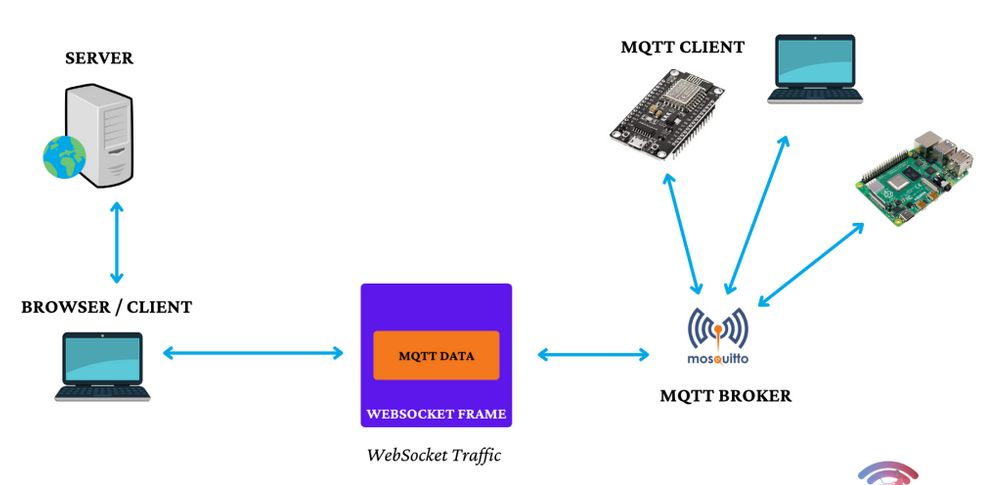
\includegraphics[scale=.6]{images/broker_server.jpg}
\caption{Server and Broker}
\end{figure}

\section{WebSockets on Windows}
\subsection*{Step 1: Install MQTT Broker on Windows}
\subsection*{Step 2: Configure the mosquitto.conf file}
You have to configure the mosquitto.conf file in your mosquitto folder. In my windows, I have setup my mosquitto.conf file in the C:\textbackslash Program Files\textbackslash mosquitto folder. Open the configuration file with Notepad++, and then add the following lines. Save your configuration file.
\\\\
By default, Port 1883 is for the MQTT Service and,
\\\\
Port 9001 is for the WebSockets

\begin{figure}[H]
\centering
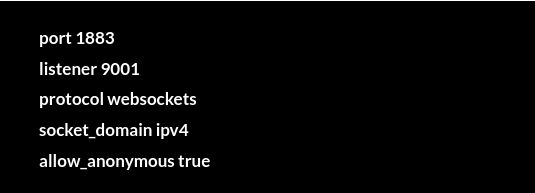
\includegraphics[scale=.8]{images/conf.jpg}
\caption{mosquitto setup on Windows}
\end{figure}

\begin{figure}[H]
\centering
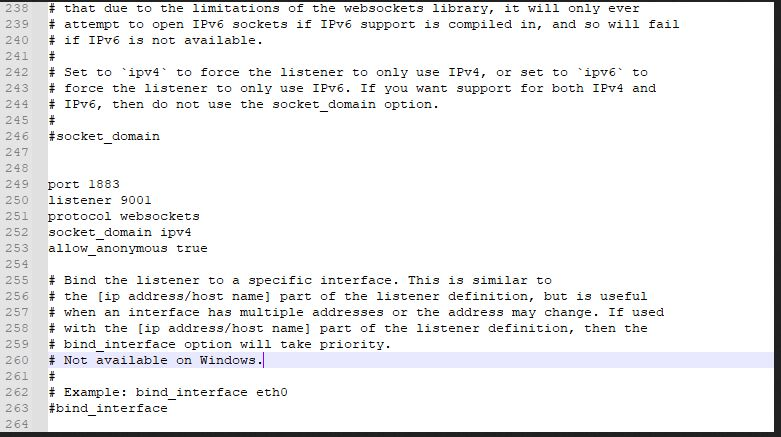
\includegraphics[scale=.8]{images/windows_setup.jpg}
\caption{mosquitto setup on Windows}
\end{figure}
mosquitto/mosquitto.conf file
\\\\
Important Note: Always check the version of mosquitto broker you are using, in this case I have used Version 2.0.14, so I needed the line, socket\_domain ipv4. Somehow I have encountered problems when using the newest version of mosquitto broker, adding that line above worked out for me. By adding this, you are forcing the listener to use IPv4.
\subsection*{Step 3: Open two ports (1883 and 9001)}
Now, you have to open the port 1883, and port 9001 on your windows machine. Basically, the ports are used to identify specific services in on your machine. For instance, the port for HTTP is 80, Netscape uses port 443 to secure the HTTP. By default, port 1883 is used by the MQTT. 
\\\\
To open the ports on your windows machine, Press Windows + R, type firewall.cpl and click Ok.
\begin{figure}[H]
\centering
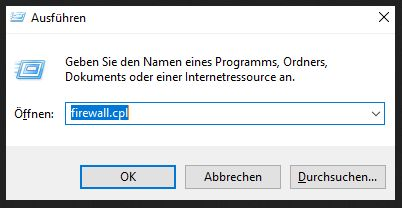
\includegraphics[scale=.6]{images/ws.jpg}
\caption{firewall.cpl}
\end{figure}
Click on Advanced Settings < Inbound Rule < New Rule
\\\\
Now, for opening a port you have to select the Rule Type as Port.
\\\\
Next, you have to select TCP or UDP Protocol, Since you are opening an MQTT port, select TCP as your protocol. Also, give specific local points, as 1883 (for MQTT).
\\\\
Under Action, select Allow Connection.
\\\\
In the Profile section, make sure everything (Domain, Private and Public) is on check.
\\\\
Under the section Name, give your port name. ( you can name anything here)
\\\\
Click Finish.
\begin{figure}[H]
\centering
\includegraphics[scale=.6]{images/Configuring_port.jpg}
\caption{Configuring port}
\end{figure}
 Go to Inbound rules, now you can see the port you have created.
 
\begin{figure}[H]
\centering
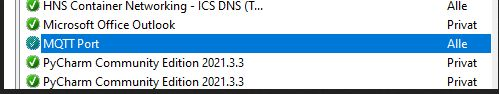
\includegraphics[scale=.6]{images/inbound_rules.jpg}
\caption{Inbound Rules}
\end{figure}
Repeat the same procedure to open the port 9001 for the WebSockets. Follow every steps except the port number as 9001 and with a different name.

\section{Connect to MQTT broker with Websocket}
\url{https://www.emqx.com/en/blog/connect-to-mqtt-broker-with-websocket}
\\\\
In recent years, with the rapid development of the Web front-end, new features of browsers are constantly emerging, more and more applications can be implemented on the browser side through the browser rendering engine. WebSocket, the instant communication method for Web applications, is also widely used.
\\\\
WebSocket is a computer communications protocol, providing full-duplex communication channels over a single TCP connection. The WebSocket protocol was standardized by the IETF as RFC 6455 in 2011, and the WebSocket API in Web IDL is being standardized by the W3C.
\subsection*{Comparison of two clients}
\subsubsection*{Paho.mqtt.js}
Paho is an MQTT client project from Eclipse, and the Paho JavaScript Client is one of the browser-based libraries that uses WebSockets to connect to the MQTT server. Compared to another JavaScript connection library, it has fewer features and is not recommended.

\subsubsection*{MQTT.js}
MQTT.js is a fully open-source client-side library for the MQTT protocol, written in JavaScript and available for Node.js and browsers. On the Node.js side, it can be installed via global installation and connected via the command line. Also, it supports MQTT/TCP, MQTT/TLS, MQTT/WebSocket connections. It is worth mentioning that MQTT.js also has good support for WeChat Mini Program.

\end{document}